% Judul dokumen
\title{Buku Tugas Akhir ITS}
\author{Musk, Elon Reeve}

% Pengaturan ukuran teks dan bentuk halaman dua sisi
\documentclass[10pt,twoside]{report}

% Pengaturan ukuran halaman dan margin
\usepackage[a5paper,top=25mm,left=25mm,right=20mm,bottom=25mm]{geometry}

% Pengaturan ukuran spasi
\usepackage[singlespacing]{setspace}

% Pengaturan format bahasa
\usepackage[indonesian]{babel}

% Pengaturan detail pada file PDF
\usepackage[pdfauthor={\@author},bookmarksnumbered,pdfborder={0 0 0}]{hyperref}

% Pengaturan jenis karakter
\usepackage[utf8]{inputenc}

% Pengaturan pewarnaan
\usepackage[table,xcdraw]{xcolor}

% Pengaturan kutipan artikel
\usepackage[numbers]{natbib}

% Package lainnya
\usepackage{changepage}
\usepackage{enumitem}
\usepackage{eso-pic}
\usepackage{etoolbox}
\usepackage{graphicx}
\usepackage{lipsum}
\usepackage{lmodern}
\usepackage{longtable}
\usepackage{tabularx}
\usepackage{wrapfig}

% Definisi untuk "Hati ini sengaja dikosongkan"
\patchcmd{\cleardoublepage}{\hbox{}}{
  \thispagestyle{empty}
  \vspace*{\fill}
  \begin{center}\textit{[Halaman ini sengaja dikosongkan]}\end{center}
  \vfill}{}{}

% Pengaturan penomoran halaman
\usepackage{fancyhdr}
\fancyhf{}
\renewcommand{\headrulewidth}{0pt}
\pagestyle{fancy}
\fancyfoot[CE,CO]{\thepage}
\patchcmd{\chapter}{plain}{fancy}{}{}
\patchcmd{\chapter}{empty}{plain}{}{}

% Pengaturan format judul bab
\usepackage{titlesec}
\titleformat{\chapter}[display]{\bfseries\Large}{BAB \centering\Roman{chapter}}{0ex}{\vspace{0ex}\centering}
\titleformat{\section}{\bfseries\large}{\MakeUppercase{\thesection}}{1ex}{\vspace{1ex}}
\titleformat{\subsection}{\bfseries\large}{\MakeUppercase{\thesubsection}}{1ex}{}
\titleformat{\subsubsection}{\bfseries\large}{\MakeUppercase{\thesubsubsection}}{1ex}{}
\titlespacing{\chapter}{0ex}{0ex}{4ex}
\titlespacing{\section}{0ex}{1ex}{0ex}
\titlespacing{\subsection}{0ex}{0.5ex}{0ex}
\titlespacing{\subsubsection}{0ex}{0.5ex}{0ex}

% Pengaturan format potongan kode
\usepackage{listings}
\definecolor{comment}{RGB}{0,128,0}
\definecolor{string}{RGB}{255,0,0}
\definecolor{keyword}{RGB}{0,0,255}
\lstdefinestyle{codestyle}{
  commentstyle=\color{comment},
  stringstyle=\color{string},
  keywordstyle=\color{keyword},
  basicstyle=\footnotesize\ttfamily,
  numbers=left,
  numberstyle=\tiny,
  numbersep=5pt,
  frame=lines,
  breaklines=true,
  prebreak=\raisebox{0ex}[0ex][0ex]{\ensuremath{\hookleftarrow}},
  showstringspaces=false,
  upquote=true,
  tabsize=2,
}
\lstset{style=codestyle}

% Isi keseluruhan dokumen
\begin{document}

  % Sampul luar
  \AddToShipoutPictureBG*{
  \AtPageLowerLeft{
    % Ubah nilai berikut jika posisi horizontal background tidak sesuai
    \hspace{-3.5mm}

    % Ubah nilai berikut jika posisi vertikal background tidak sesuai
    \raisebox{0mm}{
      
\includegraphics[width=\paperwidth,height=\paperheight]{sampul/gambar/sampul-luar.png}
    }
  }
}

% Menyembunyikan nomor halaman
\thispagestyle{empty}

% Pengaturan margin untuk menyesuaikan konten sampul
\newgeometry{
  top=95mm,
  left=25mm,
  right=20mm,
  bottom=25mm
}

\begin{flushleft}

  % Pemilihan font sans serif
  \sffamily

  % Pemilihan warna font putih
  \color{white}

  % Pemilihan font bold
  \fontseries{bx}
  \selectfont

  % Ubah penomoran buku berikut dengan yang ditentukan oleh departemen
TUGAS AKHIR - EC184801

\vspace{6ex}

% Ubah kalimat berikut dengan judul tugas akhir
\begin{large}
  APLIKASI TELEKARDIOLOGI UNTUK \textit{MOBILE ANDROID} DILENGKAPI SENSOR ECG
\end{large}

\vspace{4ex}

% Ubah kalimat-kalimat berikut dengan nama dan NRP mahasiswa
Robby Aldriyanto Raffly \\
NRP 0721 17 4000 0011

\vspace{2ex}

% Ubah kalimat-kalimat berikut dengan nama-nama dosen pembimbing
Dosen Pembimbing \\
Arief Kurniawan, ST., MT.\\
Dr. I Ketut Eddy Purnama, ST., MT.

\vspace{6ex}

% Ubah kalimat-kalimat berikut dengan nama departemen dan fakultas
DEPARTEMEN TEKNIK KOMPUTER \\
Fakultas Teknologi ELEKTRO DAN INFORMATIKA CERDAS \\
Institut Teknologi Sepuluh Nopember

% Ubah kalimat berikut dengan tempat dan tahun pembuatan buku
Surabaya 2021


\end{flushleft}

\restoregeometry


  % Sampul dalam
  \AddToShipoutPictureBG*{
  \AtPageLowerLeft{
    % Ubah nilai berikut jika posisi horizontal background tidak sesuai
    \hspace{-3.5mm}

    % Ubah nilai berikut jika posisi vertikal background tidak sesuai
    \raisebox{0mm}{
      
\includegraphics[width=\paperwidth,height=\paperheight]{sampul/gambar/sampul-dalam.png}
    }
  }
}

% Menyembunyikan nomor halaman
\thispagestyle{empty}

% Pengaturan margin untuk menyesuaikan konten sampul
\newgeometry{
  top=95mm,
  left=25mm,
  right=20mm,
  bottom=25mm
}

\begin{flushleft}

  % Pemilihan font sans serif
  \sffamily

  % Pemilihan font bold
  \fontseries{bx}
  \selectfont

  % Ubah penomoran buku berikut dengan yang ditentukan oleh departemen
TUGAS AKHIR - EC184801

\vspace{6ex}

% Ubah kalimat berikut dengan judul tugas akhir
\begin{large}
  APLIKASI TELEKARDIOLOGI UNTUK \textit{MOBILE ANDROID} DILENGKAPI SENSOR ECG
\end{large}

\vspace{4ex}

% Ubah kalimat-kalimat berikut dengan nama dan NRP mahasiswa
Robby Aldriyanto Raffly \\
NRP 0721 17 4000 0011

\vspace{2ex}

% Ubah kalimat-kalimat berikut dengan nama-nama dosen pembimbing
Dosen Pembimbing \\
Arief Kurniawan, ST., MT.\\
Dr. I Ketut Eddy Purnama, ST., MT.

\vspace{6ex}

% Ubah kalimat-kalimat berikut dengan nama departemen dan fakultas
DEPARTEMEN TEKNIK KOMPUTER \\
Fakultas Teknologi ELEKTRO DAN INFORMATIKA CERDAS \\
Institut Teknologi Sepuluh Nopember

% Ubah kalimat berikut dengan tempat dan tahun pembuatan buku
Surabaya 2021


\end{flushleft}

\restoregeometry

  \cleardoublepage

  % Pengaturan ukuran indentasi paragraf
  \setlength{\parindent}{2em}

  % Pengaturan ukuran spasi paragraf
  \setlength{\parskip}{1ex}

  % Pernyataan keaslian
  \begin{center}
  \large
  \textbf{PERNYATAAN KEASLIAN\\TUGAS AKHIR}
\end{center}

% Menyembunyikan nomor halaman
\thispagestyle{empty}

\vspace{2ex}

% Ubah paragraf-paragraf berikut sesuai dengan yang ingin diisi pada pernyataan keaslian

Dengan ini saya menyatakan bahwa isi sebagian maupun keseluruhan Tugas Akhir sada dengan judul \textbf{"Aplikasi Telekardiologi untuk Mobile Android Dilengkapi Sensor ECG"} adalah benar-benar hasil karya intelektual mandiri, diselesaikan tanpa menggunakan bahan-bahan yang tidak diijinkan da bukan karya pihak lain yang saya akui sebagai karya sendiri.

Semua referensi yang dikutip maupun dirujuk telah ditulis secara lengkap pada daftar pustaka.

Apabila ternyata pernyataan ini tidak benar, saya bersedia menerima sanksi sesuai peraturan yang berlaku.

\vspace{4ex}

\begin{flushright}
  \begin{tabular}[b]{c}
    % Ubah kalimat berikut sesuai dengan tempat, bulan, dan tahun penulisan
    Surabaya, 14 Juni 2021\\
    \\
    \\
    \\
    \\
    % Ubah kalimat-kalimat berikut sesuai dengan nama dan NRP mahasiswa
    Robby Aldriyanto Raffly\\
    0721 17 4000 0011
  \end{tabular}
\end{flushright}

  \cleardoublepage

  % Lembar pengesahan
  \begin{center}
	\large
  \textbf{LEMBAR PENGESAHAN}
\end{center}

% Menyembunyikan nomor halaman
\thispagestyle{empty}

\begin{center}
  % Ubah kalimat berikut dengan judul tugas akhir
  \textbf{DETEKSI PEJALAN KAKI PADA \textit{ZEBRACROSS} UNTUK PERINGATAN DINI PENGENDARA MOBIL MENGGUNAKAN \textit{MASK R-CNN}}
\end{center}

\begingroup
  % Pemilihan font ukuran small
  \small

  \begin{center}
    % Ubah kalimat berikut dengan pernyataan untuk lembar pengesahan
    Tugas Akhir ini disusun untuk memenuhi salah satu syarat memperoleh gelar Sarjana Teknik di Institut Teknologi Sepuluh Nopember Surabaya
  \end{center}

  \begin{center}
    % Ubah kalimat berikut dengan nama dan NRP mahasiswa
    Oleh: Agung Wicaksonoz (NRP. 0721 17 4000 0002)
  \end{center}

  \begin{center}
    % Ubah kalimat-kalimat berikut dengan tanggal ujian dan periode wisuda
    Tanggal Ujian :  Juli 2021\\
    Periode Wisuda : September 2021
  \end{center}

  \begin{center}
    Disetujui Oleh:
  \end{center}

  \begingroup
    % Menghilangkan padding
    \setlength{\tabcolsep}{0pt}

    \noindent
    \begin{tabularx}{\textwidth}{X c}
      % Ubah kalimat-kalimat berikut dengan nama dan NIP dosen pembimbing pertama
      Prof. Dr. Ir. Mauridhi Hery Purnomo, M.Eng.          & (Pembimbing I) \\
      NIP: 	19580916 198601 1 001       & ................................... \\
      &  \\
      &  \\
      % Ubah kalimat-kalimat berikut dengan nama dan NIP dosen pembimbing kedua
      Dr. Eko Mulyanto Yuniarno, S.T., M.T.     & (Pembimbing II) \\
      NIP: 19680601 199512 1 009        & ................................... \\
      &  \\
      &  \\
      % Ubah kalimat-kalimat berikut dengan nama dan NIP dosen penguji pertama
      %Dr. Galileo Galilei, S.T., M.Sc.  & (Penguji I) \\
      %NIP: 15640215 164201 1 001        & ................................... \\
      &  \\
      &  \\
      % Ubah kalimat-kalimat berikut dengan nama dan NIP dosen penguji kedua
      %Friedrich Nietzsche, S.T., M.Sc.  & (Penguji II) \\
      %NIP: 18441015 190008 1 001        & ................................... \\
      &  \\
      &  \\
      % Ubah kalimat-kalimat berikut dengan nama dan NIP dosen penguji ketiga
      %Alan Turing, ST., MT.             & (Penguji III) \\
      %NIP: 19120623 195406 1 001        & ................................... \\
    \end{tabularx}
  \endgroup

  \vspace{1ex}

  \begin{center}
    % Ubah kalimat berikut dengan jabatan kepala departemen
    Mengetahui, \\
    Kepala Departemen Teknik Komputer FTEIC - ITS \\

    \vspace{7ex}

    % Ubah kalimat-kalimat berikut dengan nama dan NIP kepala departemen
    \underline{Dr. Supeno Mardi Susiki Nugroho, ST., MT.} \\
    NIP. 19700313 199512 1 001
  \end{center}
\endgroup

  \cleardoublepage

  % Nomor halaman pembuka dimulai dari sini
  \pagenumbering{roman}

  % Abstrak Bahasa Indonesia
  \begin{center}
  \large\textbf{ABSTRAK}
\end{center}

\addcontentsline{toc}{chapter}{ABSTRAK}

\vspace{2ex}

\begingroup
  % Menghilangkan padding
  \setlength{\tabcolsep}{0pt}

  \noindent
  \begin{tabularx}{\textwidth}{l >{\centering}m{2em} X}
    % Ubah kalimat berikut dengan nama mahasiswa
    Nama Mahasiswa    &:& Agung Wicaksono \\

    % Ubah kalimat berikut dengan judul tugas akhir
    Judul Tugas Akhir &:&	Deteksi Pejalan Kaki pada \textit{Zebracross} untuk Peringatan Dini Pengendara Mobil menggunakan \textit{Mask R-CNN} \\

    % Ubah kalimat-kalimat berikut dengan nama-nama dosen pembimbing
    Pembimbing        &:& 1. Prof. Dr. Ir. Mauridhi Hery Purnomo, M.Eng. \\
                      & & 2. Dr. Eko Mulyanto Yuniarno, S.T., M.T. \\
  \end{tabularx}
\endgroup

% Ubah paragraf berikut dengan abstrak dari tugas akhir
Dewasa ini, fitur keselamatan pada kendaraan roda empat atau mobil sudah sangat berkembang pesat. Hal tersebut terbukti dengan banyaknya produsen mobil yang menerapkan teknologi seat belt, air bag, adaptive cruise control, electronic stability control, autonomous emergency braking, blind spot monitoring dan lain sebagainya. Namun, fitur yang sudah disebutkan diatas dinilai masih kurang ramah bagi pejalan kaki. Terbukti menurut data dari WHO, terdapat 270.000 pejalan kaki meninggal dunia setiap tahun atau sekitar 22\% dari seluruh korban meniggal akibat kecelakan di jalan. Berawal dari permasalahan tersebut, penulis akan melakukan penelitian mengenai pendeteksian pejalan kaki pada zebracross untuk peringatan dini pengendara mobil sebagai topik tugas akhir. Pada tugas akhir ini, terdapat 2 objek yang akan dideteksi yaitu pejalan kaki dan zebracross dengan menggunakan metode Mask R-CNN. Hasil yang diharapkan dari tugas akhir kali ini adalah terdapat model yang memiliki akurasi yang tinggi dari dataset yang tersedia yaitu Caltech Pedestrian Dataset.

% Ubah kata-kata berikut dengan kata kunci dari tugas akhir
Kata Kunci: Pejalan Kaki, \emph{Zebracross}, Mask R-CNN, Pengolahan Citra.

  \cleardoublepage

  % Abstrak Bahasa Inggris
  \begin{center}
  \large\textbf{ABSTRACT}
\end{center}

\addcontentsline{toc}{chapter}{ABSTRACT}

\vspace{2ex}

\begingroup
  % Menghilangkan padding
  \setlength{\tabcolsep}{0pt}

  \noindent
  \begin{tabularx}{\textwidth}{l >{\centering}m{3em} X}
    % Ubah kalimat berikut dengan nama mahasiswa
    \emph{Name}     &:& Elon Reeve Musk \\

    % Ubah kalimat berikut dengan judul tugas akhir dalam Bahasa Inggris
    \emph{Title}    &:& \emph{Anti-Gravity Based Energy Calculation on Outer Space Rockets} \\

    % Ubah kalimat-kalimat berikut dengan nama-nama dosen pembimbing
    \emph{Advisors} &:& 1. Nikola Tesla, S.T., M.T. \\
                    & & 2. Wernher von Braun, S.T., M.T. \\
  \end{tabularx}
\endgroup

% Ubah paragraf berikut dengan abstrak dari tugas akhir dalam Bahasa Inggris
\emph{In this research, we proposed \lipsum[1]}

% Ubah kata-kata berikut dengan kata kunci dari tugas akhir dalam Bahasa Inggris
\emph{Keywords}: \emph{Rocket}, \emph{Anti-gravity}, \emph{Energy}, \emph{Space}.

  \cleardoublepage

  % Kata pengantar
  \begin{center}
  \Large
  \textbf{KATA PENGANTAR}
\end{center}

\addcontentsline{toc}{chapter}{KATA PENGANTAR}

\vspace{2ex}

% Ubah paragraf-paragraf berikut dengan isi dari kata pengantar

Puji dan syukur kehadirat Allah SWT atas segala limpahan berkah, rahmat, serta ridho-Nya, penulis dapat menyelesaikan penelintian ini dengan judul \textbf{Deteksi Pejalan Kaki pada \textit{Zebracross} untuk Peringatan Dini Pengendara Mobil menggunakan \textit{Mask R-CNN}.}

Penelitian ini disusun dalam rangka pemenuhan bidang riset di Departemen Teknik Komputer ITS, sera digunakan sebagai persyaratan menyelesaikan pendidikan Sarjana. Penelitian ini dapat diselesaikan tidak lepas dari bantuan berbagai pihak. Oleh karena itu, penulis mengucapkan terimakasih kepada:

\begin{enumerate}[nolistsep]

  \item Keluarga, Ibu, Bapak dan Saudara tercinta yang telah memberikan dorongan baik secara spiritual dan material dalam penyelesaian buku penelitian ini. 

\end{enumerate}


\begin{flushright}
  \begin{tabular}[b]{c}
    % Ubah kalimat berikut dengan tempat, bulan, dan tahun penulisan
    Surabaya, Juni 2021\\
    \\
    \\
    \\
    \\
    % Ubah kalimat berikut dengan nama mahasiswa
    Agung Wicaksono
  \end{tabular}
\end{flushright}

  \cleardoublepage

  % Daftar isi
  \renewcommand*\contentsname{DAFTAR ISI}
  \addcontentsline{toc}{chapter}{\contentsname}
  \tableofcontents
  \cleardoublepage

  % Daftar gambar
  \renewcommand*\listfigurename{DAFTAR GAMBAR}
  \addcontentsline{toc}{chapter}{\listfigurename}
  \listoffigures
  \cleardoublepage

  % Daftar tabel
  \renewcommand*\listtablename{DAFTAR TABEL}
  \addcontentsline{toc}{chapter}{\listtablename}
  \listoftables
  \cleardoublepage

  % Nomor halaman isi dimulai dari sini
  \pagenumbering{arabic}

  % Bab 1 pendahuluan
  \chapter{PENDAHULUAN}
\label{chap:pendahuluan}

% Ubah bagian-bagian berikut dengan isi dari pendahuluan

Penelitian ini di latar belakangi oleh berbagai kondisi yang menjadi acuan. Selain itu juga terdapat beberapa permasalahan yang akan dijawab sebagai luaran dari penelitian.

\section{Latar Belakang}
\label{sec:latarbelakang}

Mobil merupakan salah satu jenis kendaraan bermotor yang banyak terdapat di Indonesia. Pada tahun 2018 Badan Pusat Statistik mencatat terdapat 16.440.987 mobil penumpang yang berada di Indonesia. Dengan bertambahnya jumlah mobil di Indonesia dari tahun ke tahun, meningkatkan juga jumlah kecelakaan mobil. Fitur keselamatan dan keamanan pada mobil sangat penting bagi para pengendara dan penumpang, sehingga para produsen mobil berusaha meningkatkan teknologi keselamatan dan keamanan pada mobil buatannya. Sebagai contoh beberapa fitur keselamatan dan keamanan yang
terdapat pada mobil antara lain, adaptive cruise control, hill strat assist, blind spot monitoring, electronic stability control dan lain sebagainya.

Menurut data dari WHO, terdapat 270.000 pejalan kaki meninggal dunia setiap tahun atau sekitar 22\% dari seluruh korban meniggal akibat kecelakan di jalan. Melihat kegiatan para pejalan kaki yang jarang berada di badan jalan, angka tersebut tentu cukup tinggi. Para pejalan kaki hanya menggunakan badan jalan ketika hendak menyebrang jalan lewat zebracross. Kelalaian dari pejalan kaki maupun pengendara mobil merupakan faktor utama mengapa angka kematian pejalan kaki cukup tinggi. Salah satu contoh kelalaian pejalan kaki adalah pada saat menyebrang jalan tidak memperhatikan kendaraan yang akan lewat dan atau melihat rambu serta lampu lalu lintas. Di sisi pengendara mobil, kelelahan,
kurangnya fokus saat berkendara dan tidak memperhatikan rambu maupun marka dapat berakibat fatal
baik kepada pejalan kaki dan pengendara lain.

Teknologi artificial intelligent sudah banyak disematkan pada mobil pada masa kini, dibuktikan
dengan adanya teknologi adaptive cruise control, hill start assist dan lain sebagainya. Artificial intelligent khususnya deep learning tentu dapat digunakan untuk deteksi pejalan kaki di zebracross guna mengurangi jumlah korban akibat kecelakaan. Deteksi pejalan kaki dapat digabungkan dengan buzzer dan atau LED sebagai komponen output untuk mengingatkan kepada pengendara bahwa ada pejalan kaki yang sedang menyebrangi jalan serta mengembalikan fokus untuk berkendara.

\section{Permasalahan}
\label{sec:permasalahan}

Cukup tingginya angka kematian pejalan kaki akibat kecelakaan lalu lintas dan belum adanya deteksi pejalan kaki di zebracross untuk peringatan dini kepada pengendara mobil. Oleh karena itu, diperlukan sebuah sistem yang mampu mendeteksi adanya pejalan kaki yang berada disekitar jalan raya untuk selanjutnya dapat digunakan sebagai peringatan kepada pengendara mobil.

\section{Tujuan}
\label{sec:Tujuan}

Berdasarkan rumusan permasalahan di atas, tujuan dari penelitian ini adalah untuk mendeteksi adanya pejalan kaki di zebracross untuk peringatan dini kepada pengendara mobil guna mengurangi angka kematian pejalan kaki akibat kecelakaan lalu lintas

\section{Batasan Masalah}
\label{sec:batasanmasalah}

Batasan-batasan dari \lipsum[1][1-3] adalah:

\begin{enumerate}[nolistsep]

  \item Mempermudah \lipsum[2][1-3]

  \item \lipsum[3][1-5]

  \item \lipsum[4][1-5]

\end{enumerate}

\section{Sistematika Penulisan}
\label{sec:sistematikapenulisan}

Laporan penelitian tugas akhir ini tersusun dalam sistematika dan terstruktur sehingga mudah dipahami dan dipelajari oleh pembaca maupun seseorang yang ingin melanjutkan penelitian ini. Alur sistematika penulisan laporan penelitian ini yaitu :

\begin{enumerate}[nolistsep]

  \item \textbf{BAB I Pendahuluan}

  Bab ini berisi uraian tentang latar belakang permasalahan, penegasan dan alasan pemilihan judul, sistematika laporan, tujuan dan metodologi penelitian.

  \vspace{2ex}

  \item \textbf{BAB II Tinjauan Pustaka}

  Pada bab ini berisi tentang uraian secara sistematis teori-teori yang berhubungan dengan permasalahan yang dibahas pada penelitian ini. Teori-teori ini digunakan sebagai dasar dalam penelitian, yaitu informasi terkait pejalan kaki, \textit{zebracross}, algoritma \textit{Mask RCNN}, dan teori-teori penunjang lainya.

  \vspace{2ex}

  \item \textbf{BAB III Desain dan Implementasi Sistem}

  Bab ini berisi tentang penjelasan-penjelasan terkait eksperimen yang akan dilakukan dan langkah-langkah pengambilan data jalan raya serta proses deteksi pejalan kaki pada \textit{zebracross}. Guna mendukung hal tersebut, digunakanlah blok diagram atau work flow agar sistem yang akan dibuat dapat terlihat dan mudah dibaca untuk implentasi pada pelaksanaan tugas akhir.

  \vspace{2ex}

  \item \textbf{BAB IV Pengujian dan Analisa}

  Bab ini menjelaskan tentang pengujian eksperimen yang dilakukan terhadap citra jalan raya, proses klasifikasi pejalan kaki dan \textit{zebracross}. Serta terkait tingkat akurasi keberhasilan pengujian yang dilengkapi dengan analisanya.

  \vspace{2ex}

  \item \textbf{BAB V Penutup}

  Bab ini merupakan penutup yang berisi kesimpulan yang di ambil dari penelitian dan pengujian yang telah dilakukan. Saran dan kritik yang membangun untuk pengembangkan lebih lanjut juga dituliskan pada bab ini.

\end{enumerate}

  \cleardoublepage

  % Bab 2 tinjauan pustaka
  \chapter{TINJAUAN PUSTAKA}
\label{chap:tinjauanpustaka}

% Ubah bagian-bagian berikut dengan isi dari tinjauan pustaka

Demi mendukung penelitian ini, \lipsum[1][1-5]

\section{Roket Luar Angkasa}
\label{sec:roketluarangkasa}

% Contoh input gambar
\begin{figure}[ht]
  \centering

  % Ubah dengan nama file gambar dan ukuran yang akan digunakan
  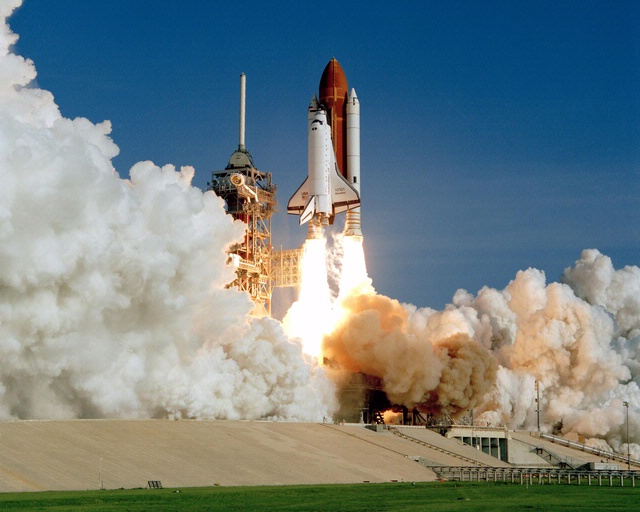
\includegraphics[scale=0.35]{gambar/roketluarangkasa.jpg}

  % Ubah dengan keterangan gambar yang diinginkan
  \caption{Peluncuran roket luar angkasa \emph{Discovery} \citep{roketluarangkasa}.}
  \label{fig:roketluarangkasa}
\end{figure}

Roket luar angkasa merupakan \lipsum[1]

\emph{Discovery}, Gambar \ref{fig:roketluarangkasa}, merupakan \lipsum[2]

\section{Gravitasi}
\label{sec:gravitasi}

Gravitasi merupakan \lipsum[1]

\subsection{Hukum Newton}
\label{subsec:hukumnewton}

Newton \citep{newton1687} pernah merumuskan bahwa \lipsum[1]
Kemudian menjadi persamaan seperti pada persamaan \ref{eq:hukumpertamanewton}.

% Contoh pembuatan persamaan
\begin{equation}
  \label{eq:hukumpertamanewton}
  \sum \mathbf{F} = 0\; \Leftrightarrow\; \frac{\mathrm{d} \mathbf{v} }{\mathrm{d}t} = 0.
\end{equation}

\subsection{Anti Gravitasi}
\label{subsec:antigravitasi}

Anti gravitasi merupakan \lipsum[1]

  \cleardoublepage

  % Bab 3 desain dan implementasi
  \chapter{DESAIN DAN IMPLEMENTASI}
\label{chap:desainimplementasi}

% Ubah bagian-bagian berikut dengan isi dari desain dan implementasi

Penelitian ini dilaksanakan sesuai dengan sistem berikut dengan implementasinya. Desain sistem merupakan konsep dari pembuatan dan perancangan infrastruktur dan kemudian diwujud kan dalam bentuk blok-blok alur yang harus dikerjakan. Pada bagian implementasi merupakan pelaksanaan teknis untuk setiap blok pada desain sistem.

\section{Deskripsi Sistem}
\label{sec:deskripsisistem}

Sistem pada tugas akhir ini merupakan implementasi dari salah satu disiplin ilmu \textit{Deep Learning} dan pengolahan citra yang berfungsi untuk mendeteksi adanya pejalan kaki yang berada di pinggir jalan, trotoar dan jalur penyebrangan. Selain pejalan kaki, deteksi juga dilakukan pada jalur penyebrangan atau \textit{zebracross} dengan tujuan untuk memberi informasi bahwa disekitar area tersebut terdapat banyak aktivitas pejalan kaki yang menyebrang jalan. Blok diagram metodologi sistem yang digunakan pada penelitian ini dapat dilihat pada Gambar \ref{fig:blok-diagram}.

\begin{figure}[ht]
	\centering
	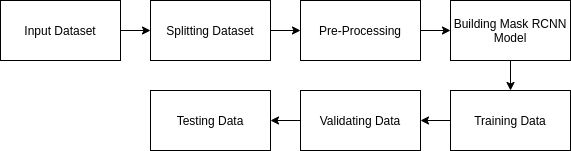
\includegraphics[scale=0.5]{gambar/blok-diagram.png}
	\caption{Blok Diagram Metodologi}
	\label{fig:blok-diagram}
\end{figure}  

\section{Pengumpulan \textit{Dataset} Gambar}
\label{sec:pengumpulandatagambar} 

Pada tugas akhir ini, \textit{dataset} yang digunakan didapatkan dengan beberapa cara, antara lain:
	\begin{enumerate}
		\item \textit{Caltech Pedestrian Database}, merupakan kumpulan gambar yang diambil dari sudut pandang pengendara mobil di California Amerika Serikat dengan ukuran 640 x 480 pixel. Terdapat sekitar 250.000 gambar dengan 350.000 \textit{bounding boxes} dan sekitar 2.300 pejalan kaki dengan kriteria unik diberi tanda. Namun, pada \textit{dataset} ini hanya pejalan kaki saja yang diberi label, sehingga perlu dilakukan proses pelabelan ulang sesuai kelas yang diinginkan. Tidak semua gambar pada \textit{dataset} ini diambil untuk digunakan, gambar yang mempunyai objek berupa pejalan kaki dan \textit{zebracross} saja yang akan digunakan. Gambar \ref{fig:caltech} merupakan contoh dari gambar yang terdapat pada \textit{Caltech Pedestrian Database}.
		\begin{figure}[ht]
			\centering
			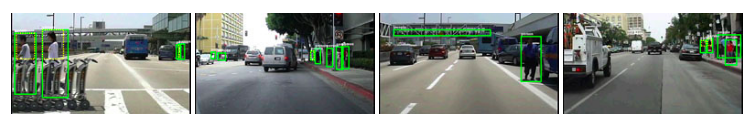
\includegraphics[scale=0.35]{gambar/caltech.png}
			\caption{Contoh Gambar dari Caltech Pedestrian Database}
			\label{fig:caltech}
		\end{figure} 
		
		\item Tangkapan layar dari beberapa video \textit{online Youtube}. Pada cara ini, penulis mencari video yang berada pada salah satu \textit{website video streaming} yaitu Youtube dengan persyaratan video diambil dari sudut pandang pengendara mobil yang berkendara pada jalan raya dengan ukuran gambar 1360x768 px. Pada \textit{frame-frame} tertentu dilakukan \textit{screenshot} dan disimpan untuk selanjutnya dilakukan proses pemberian label pada objek-objek yang diinginkan seperti pada Gambar \ref{fig:youtube-dataset}. 
		
		\begin{figure}[ht]
			\centering
			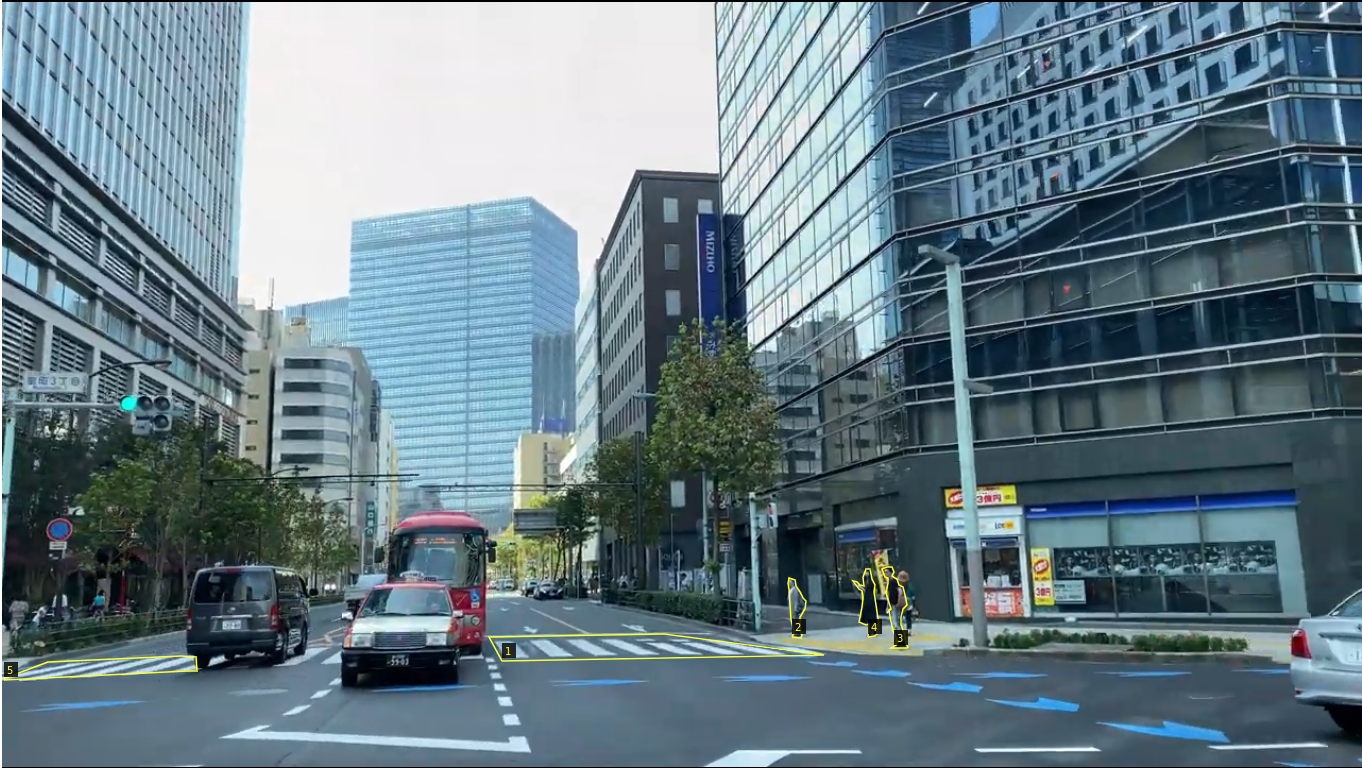
\includegraphics[scale=0.15]{gambar/youtube-dataset.png}
			\caption{Contoh Pembuatan \textit{dataset} dari \textit{Screenshot Youtube}}
			\label{fig:youtube-dataset}
		\end{figure}
		
		\item Pengambilan gambar secara mandiri menggunakan kamera \textit{smartphone} yang diambil dari sudut pandang pengendara motor dengan ukuran gambar yang diambil sebesar 1280x720 px. Pengambilan gambra dilakukan di jalan-jalan Surabaya. Setelah dilakukan pengambilan gambar, proses selanjutnya adalah pemberian label pada objek-objek yang ingin dideteksi.
	\end{enumerate}

\section{Pemisahan Data}
\label{sec:pemisahandata}

Dalam \textit{machine learning} pemisahan data ke beberapa \textit{subset} merupakan suatu hal yang sangat penting. Hal ini dikarenakan setiap \textit{subset} memiliki fungsi masing-masing. Gambar \ref{fig:data-splitting} merupakan rasio pembagian data ke masing-masing subset.

\begin{figure}[ht]
	\centering
	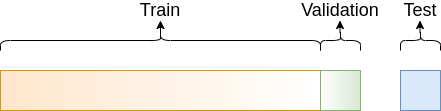
\includegraphics[scale=0.5]{gambar/data-splitting.png}
	\caption{Visualisasi Pembagian Data}
	\label{fig:data-splitting}
\end{figure}

\begin{enumerate}
	\item \textit{Training Sets}\\
	\textit{Training Sets} merupakan sampel data yang digunakan untuk melatih model yang sudah kita buat, dalam bidang \textit{Neural Network} bisa disebut juga bobot dan bias. Model yang sudah kita buat mempelajari pola masukan dan keluaran dari data ini. 
	
	\item \textit{Validation Sets}\\
	\textit{Validation Sets} merupakan sampel data yang digunakan untuk mengevaluasi model yang sudah dilatih menggunakan \textit{training sets}. Selain itu, data ini digunakan untuk memperbarui dan menyempurnakan hyperparameter dari model ke tingkat yang lebih tinggi.
	
	\item\textit{Test Sets}\\
	\textit{Test Sets} merupakan sampel data yang digunakan untuk mengevaluasi model akhir setelah melalui proses \textit{training dan validation}. Apabila pengujian model pada data ini sudah sesuai dengan yang diinginkan, maka proses \textit{learning} sudah selesai. Namun apabila pengujian tidak sesuai dengan yang diharapkan maka diperlukan pengaturan ulang mulai dari proses \textit{training}. 
\end{enumerate}

\section{\textit{Pre-Processing}}
\label{sec:preprocessing}

Pada tahap ini, gambar-gambar dari \textit{dataset} akan mengalami proses penyesuaian sebelum masuk ke proses \textit{data training}. Setiap gambar yang akan dijadikan bahan pembelajarnan model harus memiliki dimensi dan kedalaman yang sama. Tujuan dari \textit{pre processing} adalah perbaikan data gambar dengan menekan distorsi yang tidak diinginkan atau meningkatkan beberapa fitur gambar yang relevan untuk pemrosesan lebih lanjut. Gambar \ref{fig:preprocessing} merupakan tahapan dari \textit{pre-processing} gambar \textit{dataset} yang dilakukan.

\begin{figure}[ht]
	\centering
	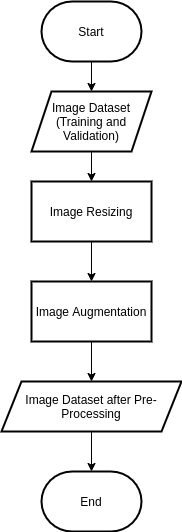
\includegraphics[scale=0.5]{gambar/flowchart-preprocessing.png}
	\caption{Diagram Alir \textit{Pre Processing}}
	\label{fig:preprocessing}
\end{figure}

Berikut merupakan penjelasan mengenai tahapan \textit{pre-processing} yang dilakukan pada tugas akhir kali ini:
\begin{enumerate}
	\item \textit{Image resizing}\\
		Langkah awal dari proses \textit{pre-processing} adalah memastikan semua gambar dalam \textit{dataset} kita memiliki ukuran yang sama. Selain itu, sama seperti sebagian besar model dari \textit{neural network} lainnya, metode yang dilakukan penulis juga mengasumsikan gambar \textit{input} berbentuk persegi. Jadi diperlukan pemeriksaan gambar di awal, apakah gambar sudah berbentuk persegi atau belum. Berbeda dari metode \textit{image resizing} pada model \textit{neural network} lainnya yang menggunakan teknik \textit{cropping} untuk membuat aspek rasio gambar input menjadi persegi, penulis menggunakan metode yang sudah terdapat pada \textit{Mask R-CNN}.
		
		Ukuran gambar yang penulis pilih pada tugas akhir kali ini adalah 512x512 pixel. Pemilihan ukuran gambar ini dilakukan untuk mengurangi beban dan waktu saat \textit{training data}. Apabila terdapat gambar pada \textit{dataset} dengan ukuran baik panjang maupun lebar lebih dari 512 pixel. maka gambar akan di \textit{down scaling} sampai ukuran 512 pixel. Sebaliknya, apabila ada gambar pada \textit{dataset} dengan ukuran lebih kecil dari 512 pixel maka akan dilakukan \textit{up scaling} sampai gambar berukuran 512 pixel. Aspek rasio gambar yang sudah melalui proses \textit{scaling} tetap dipertahankan, namun diperlukan penambahan \textit{zero padding} untuk membuat gambar \textit{input} menjadi persegi seperti yang diinginkan.
		
		\begin{figure}[ht]
			\centering
			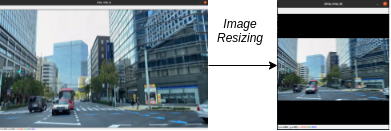
\includegraphics[scale=0.7]{gambar/image-resizing.png}
			\caption{Contoh \textit{Image Resizing}}
			\label{fig:image-resizing}
		\end{figure}
		
		Gambar \ref{fig:image-resizing} merupakan salah satu contoh \textit{image resizing} yang dilakukan. Gambar \textit{input} (gambar sebelah kiri) mempunyai ukuran 768x1360 dengan kedalaman 3 atau mempunyai format warna RGB. Setelah mengalami \textit{image resizing} (gambar sebelah kanan) ukuran gambar menjadi 290x512. Namun untuk membuat gambar memiliki aspek rasio 1:1 (berbetuk persegi) maka diperlukan penambahan \textit{zero padding} pada bagian atas gambar sebesar 111 pixel dan pada bagian bawah gambar sebesar 111 pixel. Dengan penambahn \textit{padding} seperti itu membuat gambar \textit{input} berbentuk persegi namun tidak mengurangi informasi gambar. 
		   
	\item \textit{Image Augmentation}\\
	Langkah selanjutnya pada \textit{pre-processing} adalah \textit{image augmentaion}. Proses augmentasi yang dilakukan pada tugas akhir ini adalah rotasi dan transformasi. Tujuan dari penggunanaan \textit{image augmentation} adalah untuk mengekspos \textit{neural network} ke berbagai variasi, agar dapat mengenali fitur yang akan dilakukan pada proses \textit{training}. Hal tersebut akan sangat membantu \textit{neural network} untuk mengenali variasi yang tidak terdapat pada dataset. Seperti yang terdapat pada Gambar \ref{fig:image-augmentation}, tanpa ada augmentasi maka \textit{neural network} hanya mengenali satu kondisi saja. Jika memakai augmentasi gambar seperti transformasi, maka setidaknya \textit{neural network} akan dapat mengenali 2 kondisi. Semakin banyak augmentasi yang digunakan semakin banyak pula kondisi yang bisa dikenali oleh \textit{neural network}. Namun semakin banyak kondisi yang dikenali, semakin lama dan berat proses \textit{training data} yang dilakukan. 
	
	\begin{figure}[ht]
		\centering
		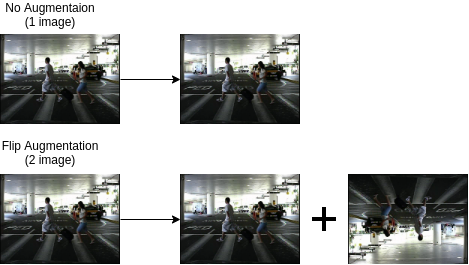
\includegraphics[scale=0.5]{gambar/image-augmentation.png}
		\caption{Contoh \textit{Image Augmentation}}
		\label{fig:image-augmentation}
	\end{figure}
	  
\end{enumerate}

\section{Membangun Model Mask R-CNN
\label{sec:membangunmodelmaskrcnn}}



\section{Implementasi Alat
\label{sec:implementasi alat}}

Alat diimplementasikan dengan \lipsum[1]

% Contoh pembuatan potongan kode
\begin{lstlisting}[
  language=C++,
  caption={Program halo dunia.},
  label={lst:halodunia}
]
#include <iostream>

int main() {
    std::cout << "Halo Dunia!";
    return 0;
}
\end{lstlisting}

\lipsum[2-3]

% Contoh input potongan kode dari file
\lstinputlisting[
  language=Python,
  caption={Program perhitungan bilangan prima.},
  label={lst:bilanganprima}
]{program/bilangan-prima.py}

\lipsum[4]

  \cleardoublepage

  % Bab 4 pengujian dan analisis
  \chapter{PENGUJIAN DAN ANALISIS}
\label{chap:pengujiananalisis}

% Ubah bagian-bagian berikut dengan isi dari pengujian dan analisis

Pada penelitian ini dipaparkan \lipsum[1][1-5]

\section{Skenario Pengujian}
\label{sec:skenariopengujian}

Pengujian dilakukan dengan \lipsum[1-2]

\section{Evaluasi Pengujian}
\label{sec:analisispengujian}

Dari pengujian yang \lipsum[1]

% Contoh pembuatan tabel
\begin{longtable}{|c|c|c|}
  \caption{Hasil Pengukuran Energi dan Kecepatan}
  \label{tb:EnergiKecepatan}\\
  \hline
  \rowcolor[HTML]{C0C0C0}
  \textbf{Energi} & \textbf{Jarak Tempuh} & \textbf{Kecepatan} \\
  \hline
  10 J & 1000 M & 200 M/s \\
  20 J & 2000 M & 400 M/s \\
  30 J & 4000 M & 800 M/s \\
  40 J & 8000 M & 1600 M/s \\
  \hline
\end{longtable}

\lipsum[2-4]

  \cleardoublepage

  % Bab 5 penutup
  \chapter{PENUTUP}
\label{chap:penutup}

% Ubah bagian-bagian berikut dengan isi dari penutup

\section{Kesimpulan}
\label{sec:kesimpulan}

Berdasarkan hasil pengujian yang \lipsum[1][1-3] sebagai berikut:

\begin{enumerate}[nolistsep]

  \item Pembuatan \lipsum[2][1-3]

  \item \lipsum[2][4-6]

  \item \lipsum[2][7-10]

\end{enumerate}

\section{Saran}
\label{chap:saran}

Untuk pengembangan lebih lanjut pada \lipsum[1][1-3] antara lain:

\begin{enumerate}[nolistsep]

  \item Memperbaiki \lipsum[2][1-3]

  \item \lipsum[2][4-6]

  \item \lipsum[2][7-10]

\end{enumerate}

  \cleardoublepage

  % Daftar pustaka
  \renewcommand\bibname{DAFTAR PUSTAKA}
  \addcontentsline{toc}{chapter}{\bibname}
  \bibliographystyle{unsrtnat}
  \bibliography{pustaka/pustaka.bib}
  \cleardoublepage

  % Biografi penulis
  \begin{center}
  \Large
  \textbf{BIOGRAFI PENULIS}
\end{center}

\addcontentsline{toc}{chapter}{BIOGRAFI PENULIS}

\vspace{2ex}

\begin{wrapfigure}{L}{0.3\textwidth}
  \centering
  \vspace{-3ex}
  % Ubah file gambar berikut dengan file foto dari mahasiswa
  
\includegraphics[width=0.3\textwidth]{gambar/elon.jpg}
  \vspace{-4ex}
\end{wrapfigure}

% Ubah kalimat berikut dengan biografi dari mahasiswa
Elon Reeve Musk, lahir pada \lipsum[1]

\lipsum[2]

  \cleardoublepage

\end{document}
